\documentclass[11pt]{article}
\usepackage[utf8]{inputenc}
\usepackage{amsmath}
\usepackage[margin=2cm,top=0.5cm]{geometry}
\usepackage{amsfonts}
\usepackage{bbold}
\usepackage{tcolorbox}
\usepackage{graphicx}
\usepackage[]{algorithm2e}

\title{Crossentropy}
\author{Remi Boutin}
\date{June 2019}

\begin{document}

\maketitle

\section{Crossentropy is just the likelihood}

Let's assume $\mathbf{D} =  \left\{(X_i,Y_i), i=1,...,n \right\}$ our i.i.d observations such that :  
$ (y_1,...,y_n) $ is an i.i.d sample draw from the TRUE distribution $\mathrm{P}$. We define the following for our classes $c$ with $c=1,...,K$  :

\begin{equation}
\begin{split}
k_c & := \sum_{i=1}^{N} \mathbb{1}_{y_i=c}\\ 
p_c & := \frac{k_c}{N}\\
\hat{k}_c & := \sum_{i=1}^{N} \mathbb{1}_{\hat{y}_i=c}\\
\hat{p}_c & := \frac{\hat{k}_c}{N} 
\end{split}
\end{equation}

We can now calculate the likelihood of our data according to the estimated probabilities (the model) : 

\begin{equation}
\begin{split}
    \mathbb{P}( Y_1=y_1,...,Y_n=y_n | model) & = \prod_{i=1}^{N} \mathrm{p}( y_i | model)\\
    & =  \prod_{i=1}^{N}  \hat{p}_{y_i}\\
    & =  \prod_{C=1}^{K} \hat{p}_{c}^{k_c}
\end{split}
\end{equation}
Let's take the log likelihood :
\begin{equation}
    l(y_1,...,y_n| model) = \sum_{c=1}^{K} k_c \log(\hat{p}_{c})
\end{equation}
Dividing by $N$ and multiplying by $-1$ gives us : 

\begin{equation}
    - \frac{1}{N}l(y_1,...,y_n| model)  = - \frac{1}{N} \sum_{c=1}^{K} k_c \log(\hat{p}_{c})
     = - \sum_{c=1}^{K} p_c \log(\hat{p}_{c}) := H(\mathrm{P},\mathrm{Q})
\end{equation}
where $\mathrm{Q}$ corresponds to the estimated distribution.\vskip 1\baselineskip 

\section{Crossentropy in Deep Learning}

Now that we understand the cross entropy as a mean to compare two distributions (between $p$ the real distribution of the categories and $q$ defined by the estimated $\hat{p}_c$), let's take a look at its evaluation during the training of the model.

\subsection{Evaluation of the lost}
We suppose here that the categories are encoded as a one hot encoded vector, that is,
a vector $c = [0,..,1,0,..,0]$ with one on the position corresponding to the right category of the observation and zero otherwise. To relate to the previous section, we now have :
$$
p_c = \left\{
    \begin{array}{ll}
        1 & \mbox{if }  y = c \\
        0 & \mbox{otherwise}
    \end{array}
\right.
$$
We write ${L(f(x) , y) }$ instead of ${L(q,p)}$ since $q(|x) = f(x)$ and $ p(|x) = y$, once it has been "one hot encoded". Therefore, the loss evaluated on one observation gives us:
\begin{equation}
\end{equation}

\begin{equation} \label{eq1}
\begin{split}
    {L(f(x) , y) } & = - \sum_c p_c * log( q_c)\\
     & =  - log( q_{\text{real categ}})
\end{split}
\end{equation}
The loss only evaluates the probability the model gives to the real category of your observation. But since $\sum_c p_c = 1 $, it changes the whole distribution. \par
A quick look at the function $f : x \mapsto - log(x) $ give a good insight on how the estimated probability affect the loss function (or not): 

\begin{figure}[h]
    \centering
    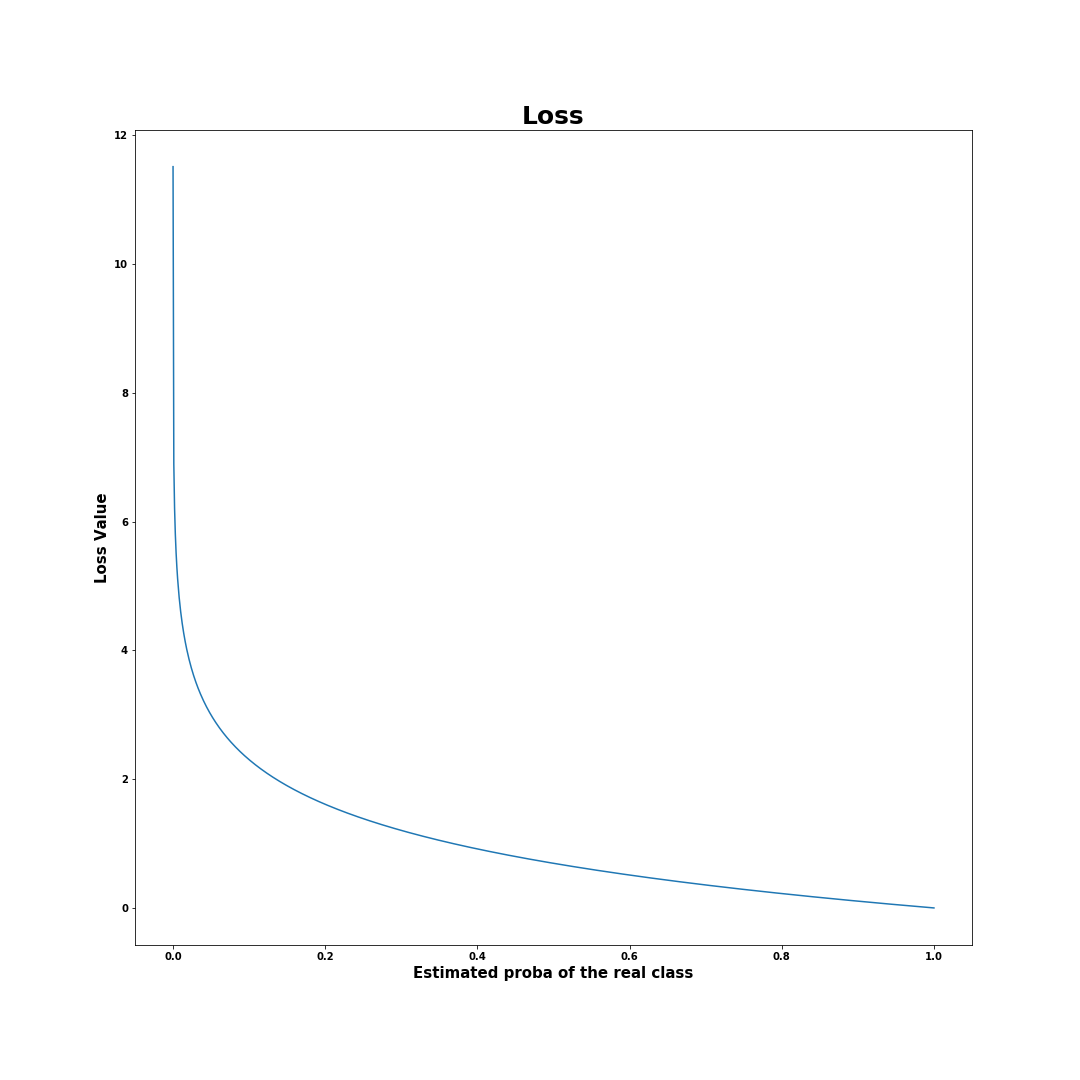
\includegraphics[width=10cm]{crossentropy_1d.png}
    \caption{Impact of the estimated probability of the real class on the loss}
    \label{fig:crossentropy_1d}
\end{figure}
\newpage




\subsection{Pseudo-code of how it works step by step}
\begin{itemize}
    \item E = Number of epochs 
    \item B = Number of batches per epochs
    \item $B(b) = \{(x,y) \in \text{batch b at the epoch considered}\}$, we don't specify the epoch for the sake of clear reading
    \item $n_b $ = batch size
\end{itemize}

\textcolor{red}{NEED TO IMPROVE : DETAILS ON THE BACK-PROPAGATION ALGORITHM.  USE $\tilde{p}_c(\theta)$ AND DO THE DERIVATION OF THE SOFTMAX FUNCTION ! }


\begin{tcolorbox}[colback = white, sharp corners=all]
\begin{algorithm}[H]
 Initialization\;
 \For{epoch = 1 to E}{
    \For{b = 1 to B}{
    \begin{equation}
    \begin{split}
        c(b) & = \frac{1}{n_b} \sum_{(x,y)\in B(b)}{L(f(x) , y) }\\
             & = - \frac{1}{n_b} \sum_{(x,y)\in B(b)}  log( \tilde{p}_{\text{c}}) \hspace{19} \text{where c is the real class of the input }
    \end{split}
    \end{equation}
    \text{Perform back-propagation with cost c(b)}
    }
 }
\caption{Step by step cross entropy}
\end{algorithm}
\end{tcolorbox}



\end{document}